%%% template.tex
%%%
%%% This LaTeX source document can be used as the basis for your technical
%%% paper or abstract. Intentionally stripped of annotation, the parameters
%%% and commands should be adjusted for your particular paper - title, 
%%% author, article DOI, etc.
%%% The accompanying ``template.annotated.tex'' provides copious annotation
%%% for the commands and parameters found in the source document. (The code
%%% is identical in ``template.tex'' and ``template.annotated.tex.'')

\documentclass[]{acmsiggraph}
\usepackage{algorithm}
\usepackage[noend]{algpseudocode}
\TOGonlineid{45678}
\TOGvolume{0}
\TOGnumber{0}
\TOGarticleDOI{0}
\TOGprojectURL{}
\TOGvideoURL{}
\TOGdataURL{}
\TOGcodeURL{}
\usepackage{color}
%\definecolor{red}{rgb}{0.9, 0.17, 0.31}
\usepackage{multirow}
\usepackage{subfig}
\usepackage{xcolor}
\usepackage{lipsum}
\usepackage{listings}
\usepackage{graphicx}
\usepackage{glsllst} % My own package providing markup listing for glsl
\usepackage{rmlst}   % My own package providing markup listing for renderman
\usepackage{amsmath}
\usepackage{hyperref}

\lstset{
	backgroundcolor=\color[rgb]{0.95, 0.95, 0.95},
	tabsize=3,
	%rulecolor=,
	basicstyle=\footnotesize\ttfamily,
	upquote=true,
	aboveskip={1.5\baselineskip},
	columns=fixed,
	showstringspaces=false,
	extendedchars=true,
	breaklines=true,
	prebreak = \raisebox{0ex}[0ex][0ex]{\ensuremath{\hookleftarrow}},
	frame=none,
	aboveskip=15pt,
	belowskip=8pt,
	captionpos=t,
	showtabs=false,
	showspaces=false,
	showstringspaces=false,
	identifierstyle=\ttfamily,
	%keywordstyle=\color{red}\bfseries,
	%keywordstyle=[1]\bfseries\color{syntaxBlue},
	%keywordstyle=[2]\bfseries\color{syntaxRed},
	%keywordstyle=[3]\color{blue}\bfseries,
	%keywordstyle=[4]\bfseries\color{syntaxBlue},
	commentstyle=\color[rgb]{0.082,0.639,0.082},
	keywordstyle=[1]\bfseries\color[rgb]{0,0,0.75},
	keywordstyle=[2]\bfseries\color[rgb]{0.5,0.0,0.0},
	keywordstyle=[3]\bfseries\color[rgb]{0.127,0.427,0.514},
	keywordstyle=[4]\bfseries\color[rgb]{0.4,0.4,0.4},
	stringstyle=\color[rgb]{0.639,0.082,0.082},
}

\title{Principles of Rendering: Criminowl}

\author{Jack Diver\thanks{e-mail:jackdiver@hotmail.co.uk}\\National Centre for Computer Animation}
\pdfauthor{Jack Diver}

\keywords{rendering}

\begin{document}

\maketitle


\begin{abstract}
This paper will explore rendering techniques, using procedural Shaders and GLSL API. The aim was to create a photo realistic image of an object small enough to hold in your hand, using real time rendering techniques.
\end{abstract}
%\keywordlist
%\TOGlinkslist

\section{Introduction} \label{sec:introduction}
I am attempting to create a brushed and oiled wood shader, with a large degree of wear. This material is found on a small carved owl and consists of several layers, all some form of noise which is relatively simple, but together create a detailed surface. 

\begin{figure}[htbp]\centering
 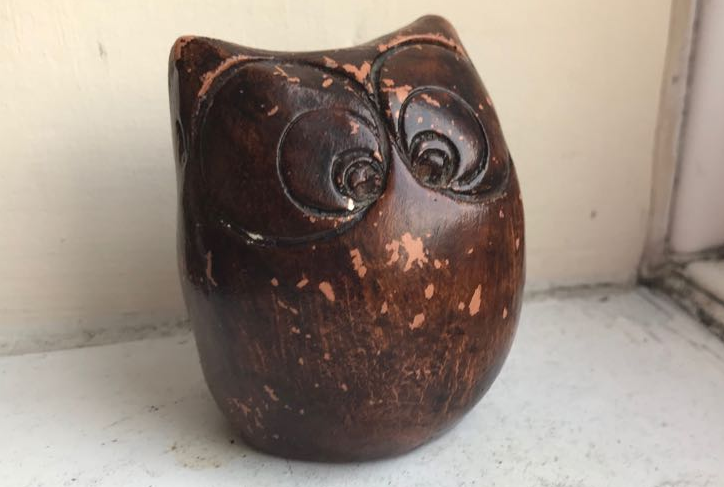
\includegraphics[width=0.7\linewidth]{images/real.png}
 \caption{\label{fig:reference}Photo of the carved owl.}
\end{figure}

I observed these properties from the owl:
\begin{enumerate}
 \item Large carved circles for the eyes.
 \item Variation in the base colour from dark to light brown.
 \item A brushed pattern that shows up more in the light areas
 \item Small and frequent rough scratches.
 \item Larger, less frequent and vein-like scratches.
 \item Lots of chips in the painted coats.
\end{enumerate}

I envisioned the owl as a hero character, and also aimed to animate him. I ported some of the noise functions from a procedural OSL shader that I created prior to this, and used them as the basis for my surface patterns.  

\section{Method Overview} \label{sec:overview}
\subsection{Eyes}
I began by writing a concentric circle shader, which borrows \textit{smoothpulse} and \textit{smoothpulsetrain} from Larry Gritz \cite{larrygritzarman}. These functions produce a repeating pattern of smooth steps up and then down, similar to a sin wave but with flat peaks and dips. A \textit{smoothpulse} is defined by subtracting or multiplying two \textit{smoothsteps} \cite{fundza}. I used the position vector to calculate distance from the origin, this is useful as all points lying on the edge of a circle are the same distance from the centre of that circle.
\begin{algorithm}
\caption{Concentric Circles}\label{alg:concircles}
\begin{algorithmic}[1]
\Procedure{Concentric}{$p, f, g, t$}
\State $r\gets \sqrt[]{p.x^2 + p.y^2}$\Comment{Get the distance from origin}
\State $sum\gets (p.x + p.y)/r$\Comment{Sum the normalized x and y}
\State $period \gets g * sum$
\State \textbf{return} $spte(t, t + period, f, period, r)$
\EndProcedure
\end{algorithmic}
\end{algorithm}
\newline 
Note that \textit{spte} is a wrapper for Larry Gritz function that applies the same fuzz to each side of the \textit{smoothpulse}. The circles in the eye are not concentric, they all share a single point. The circles do not grow linearly; their growth is exponential. To account for these properties I added two new parameters to the algorithm, a warp factor, and an exponent. When warp is zero we get concentric circles, when it is one we get the eye pattern. Exponent determines the growth factor of the circles.
\begin{algorithm}
\caption{Owl eye}\label{alg:owleye}
\begin{algorithmic}[1]
\Procedure{Eye}{$p, f, g, t, w, e$}
\State $recip \gets 1/e$ \Comment{Get the reciprocal of the exponent}
\State $r\gets \sqrt[]{p.x^2 + p.y^2}$\Comment{Get the distance from origin}
\State $sum\gets (p.x + p.y)/r$\Comment{Sum the normalized x and y}
\State $period \gets g * lerp(1, pow(sum,recip), w)$
\State \textbf{return} $spte(t, t + period, f, period, pow(r, recip))$
\EndProcedure
\end{algorithmic}
\end{algorithm}
\newline
 Here we make several modifications, to warp the circles away from being concentric we linearly interpolate between a uniform gap, and $sum^{recip}$ which is what gives us the shared point. Similarly we use $r^{recip}$ as the final parameter to our \textit{smoothpulsetrain} which is what gives us the non-linear growth.
On top of this, noise was added to the return value, and the position p, to give a more natural and imperfect result.

To perform the displacement I added geometry, tessellation control, and tessellation evaluation stages into my shader. The tessellation control used an expanded version of the mask used for the eyes, to only tessellate the geometry in the areas that would be displaced. The tessellation uses subroutines to allow the user to switch between different tessellation types, currently flat tessellation and phong tessellation are offered. Flat tessellation was performed by simply assigning positions to the new vertices using their bary-centric coordinates to blend between the positions of the parent vertices. Phong tessellation was used \cite{Boubekeur:2008:PhongTess}, which first projects the vertex onto the three tangent planes of the parent vertices, then blends the resulting projections using bary-centric coordinates as we did with flat tessellation. I also added a uniform that allows the user to blend between flat and phong tessellation which means that they can get a smooth tessellation. 

\begin{figure}[htbp]
  \centering
 \subfloat[Flat tessellation]{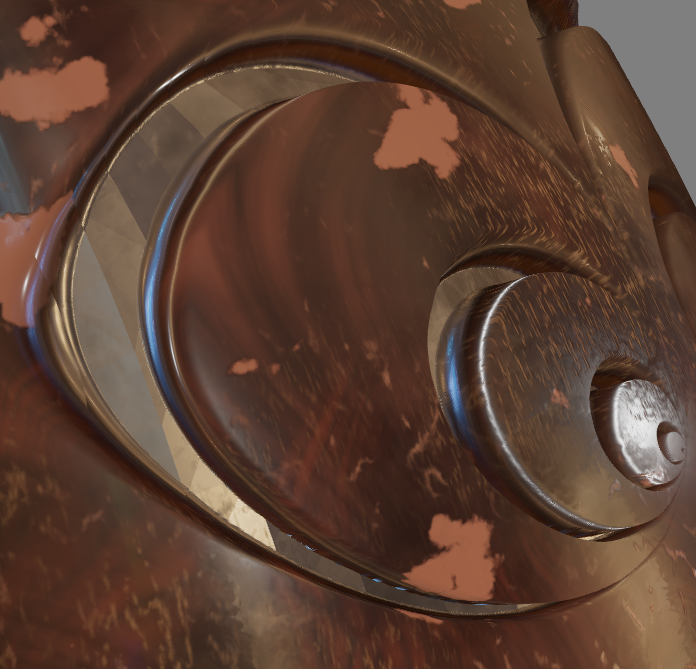
\includegraphics[width=0.32\linewidth]{images/eye_tess_flat.png}}
 \hfill
 \subfloat[Phong tessellation]{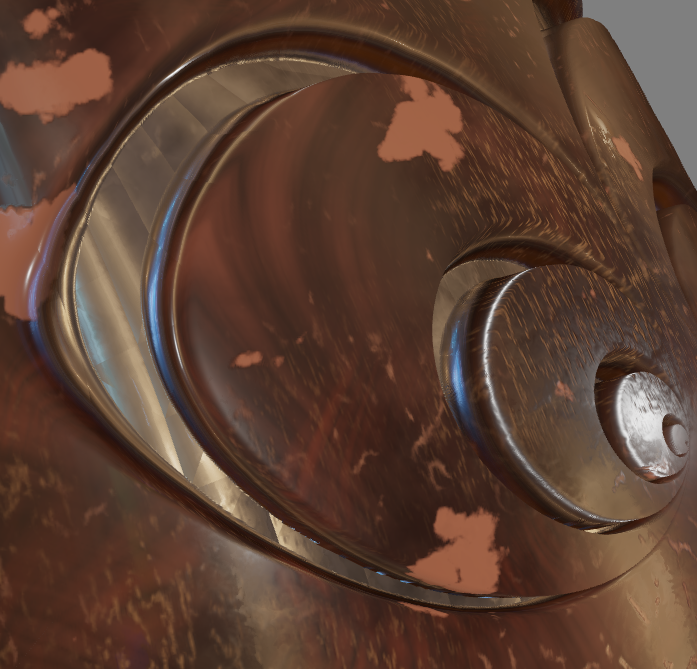
\includegraphics[width=0.32\linewidth]{images/eye_tess_phong.png}}
 \hfill
 \subfloat[Blended tessellation]{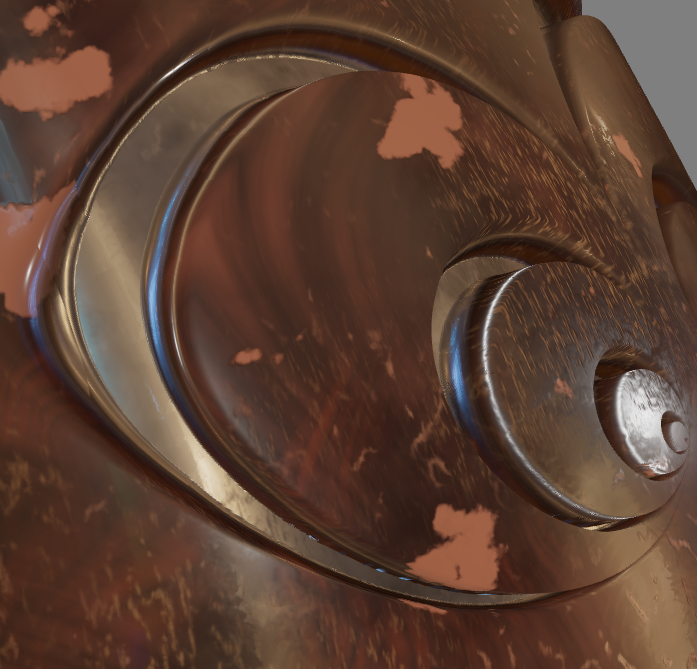
\includegraphics[width=0.32\linewidth]{images/eye_tess_blend.png}}
\end{figure}

\subsection{Wood}

The wood texture is essentially lots of different types of noise mixed together. I used a large low frequency noise to blend the layers and turbulence was also used frequently. To produce the paint chips I defined a \textit{slicednoise} function, which capped the noise at a given value using \textit{smoothstep}. I found that this is very useful for blending my other layers together as most of them are limited to a few spots on the surface. The brush marks were created using turbulence, with noise and y-axis scaling applied to the position. The stretching produced long strands similar to brush marks. I defined another function which was used in the creation of the rough wood cracks and also the veins. This function again  applies scaling in the y-axis to position, but then uses the \textit{slicednoise} function I described earlier; we subtract the return of that function from one, which results in thin lines. These lines are the gaps between the spots of noise created by \textit{slicednoise}. We also get lots of thin, faint lines within the spots themselves.

\subsection{3D Textures}

\subsubsection{Albedo}

Most of my methods involve the use of 3D noise to give proceduralism to the shader, however many successive calls to generate noise significantly hurt my performance so I decided to bake the layers of noise into a 3D texture. To do this I moved my code into a new shader, and setup a unit plane with orthographic projection, I then created a 3D texture and rendered to 2D slices of that texture using a frame buffer. Where each slice that was rendered, was given a z-depth value through a uniform, that offset the noise. Doing this increased my main shaders performance, however had several draw-backs, such as very high memory consumption which led to reduced resolutions, and also the user lost the ability to change the surface colour at runtime (unless they generated multiple maps).

\begin{figure}[htbp]
  \centering
 {
\includegraphics[width=0.24\linewidth]{images/albedo_slice_01.jpg}}
 \hfill
 {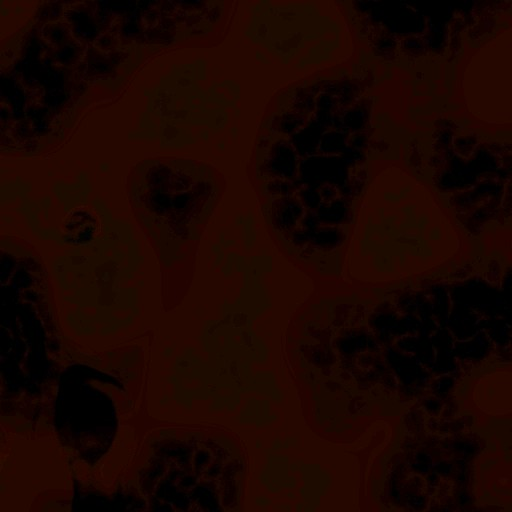
\includegraphics[width=0.24\linewidth]{images/albedo_slice_02.jpg}}
 \hfill
 {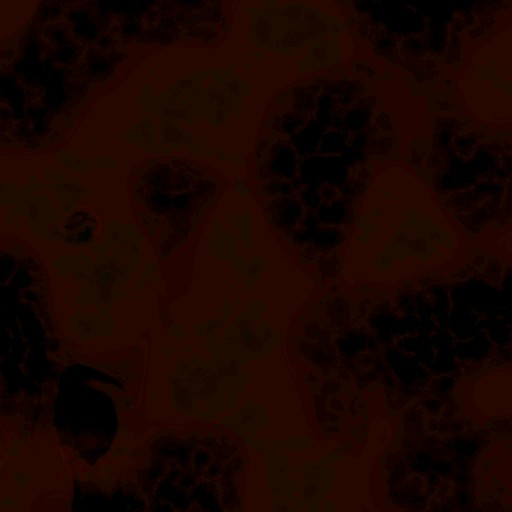
\includegraphics[width=0.24\linewidth]{images/albedo_slice_03.jpg}}
 \hfill
 {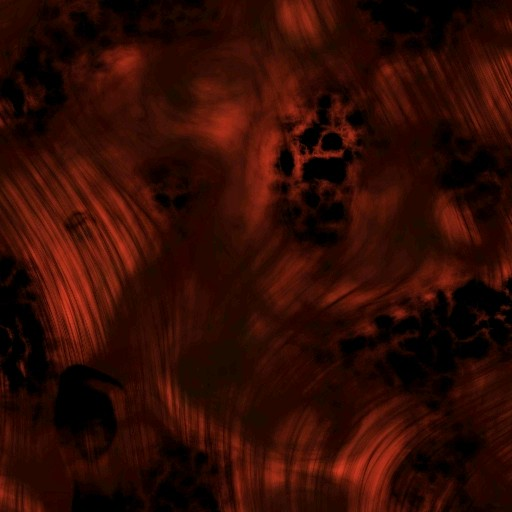
\includegraphics[width=0.24\linewidth]{images/albedo_slice_04.jpg}}
 \vskip 0.2em
 {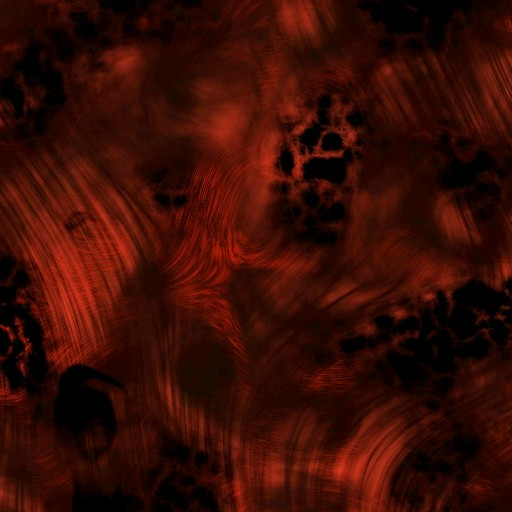
\includegraphics[width=0.24\linewidth]{images/albedo_slice_05.jpg}}
 \hfill
 {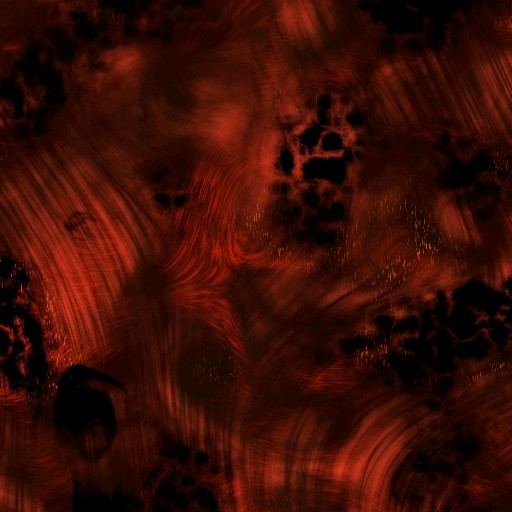
\includegraphics[width=0.24\linewidth]{images/albedo_slice_06.jpg}}
 \hfill
 {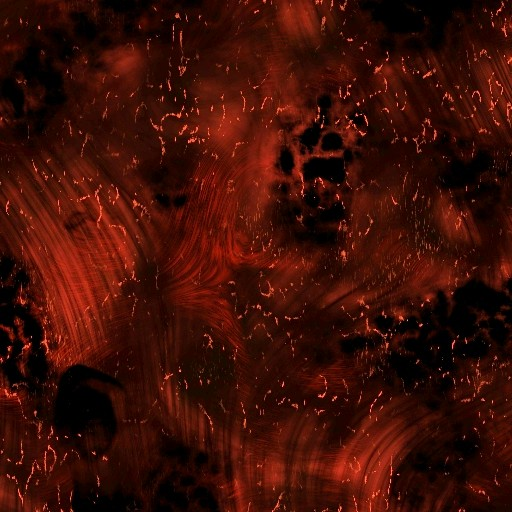
\includegraphics[width=0.24\linewidth]{images/albedo_slice_07.jpg}}
 \hfill
 {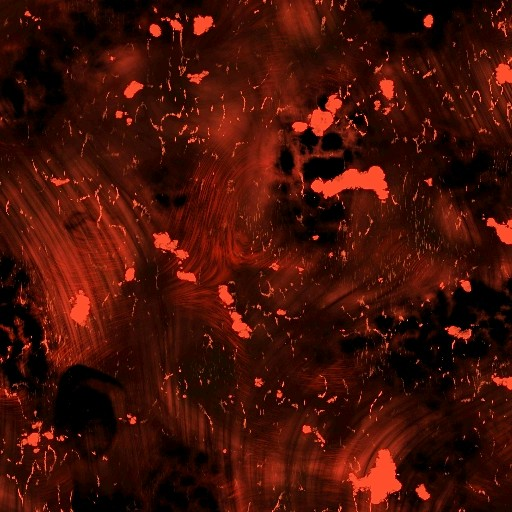
\includegraphics[width=0.24\linewidth]{images/albedo_slice_08.jpg}}
  \caption{\label{fig:albedo}Shows the layers of noise used to build up the albedo texture, this is a slice of the 3D texture.}
\end{figure}

\subsubsection{Normals}

The generation of the 3D albedo map used float values from noise to blend colours together. In the original OSL shader, I summed these float values to use as my surface displacement, and so to keep this I stored the sum in the W component of the albedo texture. I didn't want to displace the surface of the owl in the same way as I did for the eyes as this would create very dense geometry and slow down performance, instead I wanted to use bump mapping. Bump mapping with a grey scale height map uses finite difference which involves at least four texture look-ups, seeing as the surface displacement is unchangeable due to it being baked previously, I decided to also bake my normal map, as this would reduce my texture look-ups. I used a very similar method to the one described for the albedo map, however this time the shader being rendered computed the finite difference between the W components of texels offset from the current fragment. 

\begin{figure}[htbp]
  \centering
 {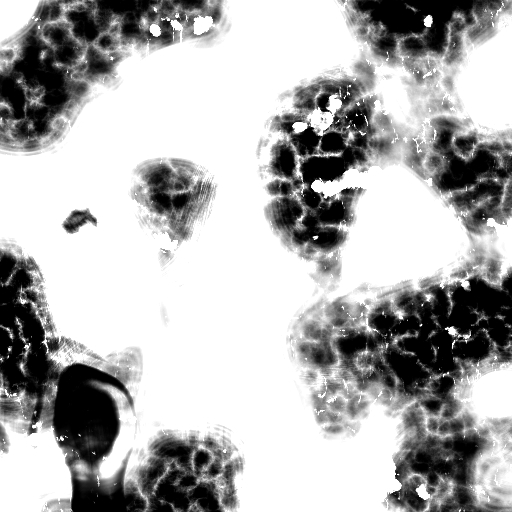
\includegraphics[width=0.46\linewidth]{images/height_slice.jpg}}
 \hfill
 {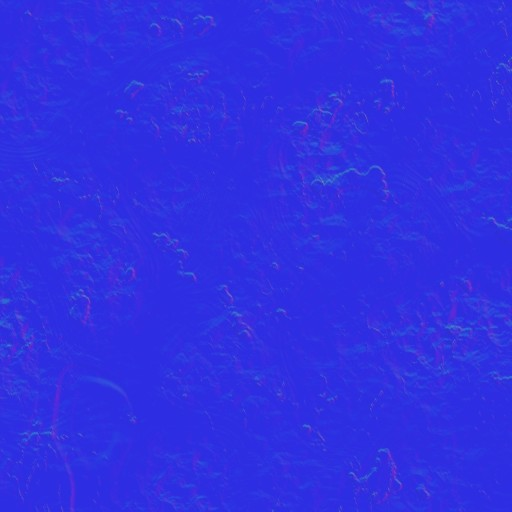
\includegraphics[width=0.46\linewidth]{images/normal_slice.jpg}}
  \caption{\label{fig:normals}Slice of the 3D height map on the left, and on the right is the normal map generated for it through finite difference.}
\end{figure}

\subsection{Animation}

To animate the owl, I first created a rig for the owl (with much help from Miguel Goncalves), then key-framed some poses. I then exported an obj sequence of the entire animation. I wanted to be able to have no limits on the amount of poses that could be provided for the object, and so I decided to use a shader storage buffer object, as these can be as large as the GPU memory available. In my C++ code, I loaded all of the obj's, and then copied their vertex positions and normals into one large array. The positions and normals were padded to be four floats in size as there are alignment issues with passing vector3's. Instead of storing difference from the rest position, I just passed the absolute positions of every frame as this simplified my code. I then passed a blend float through a uniform, which could be in the range 0 to (N-1), where N is the number of frames, I then used this to smoothstep between floor(blend) and ceil(blend). To correctly index into my SSBO I also passed the target size, which was the amount of elements occupied by one morph target, and I also passed the normal offset, which represented how far into the SSBO, my normal data began. In the demo I am using 200 morph targets.

An issue I faced with this method was that the 3D positions used for texture look-up and to calculate the eyes, were now moving and this made the owl look like it was sliding through the textures. To resolve this I passed the base position and normals through the shader pipeline along with the morphed ones, but only used the base ones for texture look-up and eye calculations.

\subsection{Shading and reflectance model}

I implemented the Physically based, Cook-Torrence shading model. I chose to use Trowbridge-Reitz GGX that is also used by Epic \cite{epicpbr}, as it was well documented in their course notes. I also used the Schlick GGX, geometric shadowing matched to Smith, as this was in the course notes and also very efficient. The Fresnel is also Schlick. I then implemented image based lighting which gave a huge visual boost, this was done by converting a HDR spherical map into a cube map, by rendering each face to texture using a framebuffer and projection shader. Next I convoluted the resulting cube map, using importance sampling to create an irradiance map.
Then I then used a split sum approximation detailed by Epic to generate a BRDF map and a pre-filtered environment map, that stores varying roughness levels inside of it's mip-maps. Joey De Vries explains the entire process very well \cite{specibl}.

\begin{figure}[htbp]
 \centering
 \subfloat[Looking surprised]{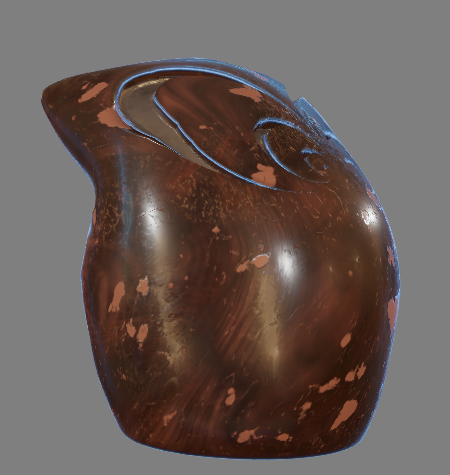
\includegraphics[width=0.49\linewidth]{images/morph_01.png}}
 \hfill
 \subfloat[Looking sad]{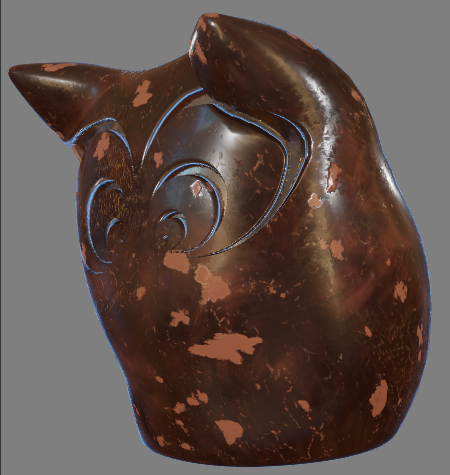
\includegraphics[width=0.49\linewidth]{images/morph_02.png}}
 \caption{\label{fig:morph}Two of the key poses from the animation sequence.}
\end{figure}

\section{Results} \label{sec:results}
The images on the right show some of the results that can be achieved with the shader parameters.

There are several aspects of this shader that I would improve on. The first would be to improve the memory footprint, by using some method such as sparse textures, to turn my 3D textures into voxels, and only store the ones that intersect with my geometry. I would also have liked to generate an Ambient occlusion map as this would have improved the self shadowing. I would also have improved on my placement of the wood chips by biasing them around the eyes. Overall I am happy with my results, especially the customisablity achieved through the shader parameters, that can be leveraged to make interesting results.

\begin{figure}[tp]
 \centering
 \subfloat[Trying to match the object]{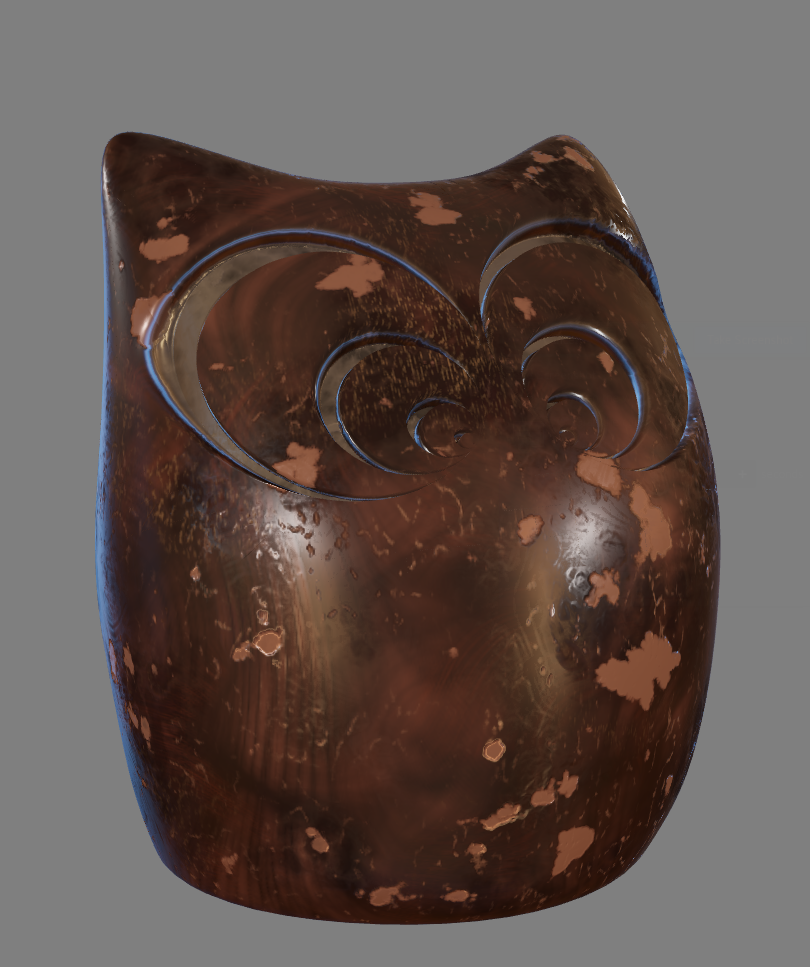
\includegraphics[width=0.49\linewidth]{images/result_base.png}}
 \hfill
 \subfloat[Morphed and high spec]{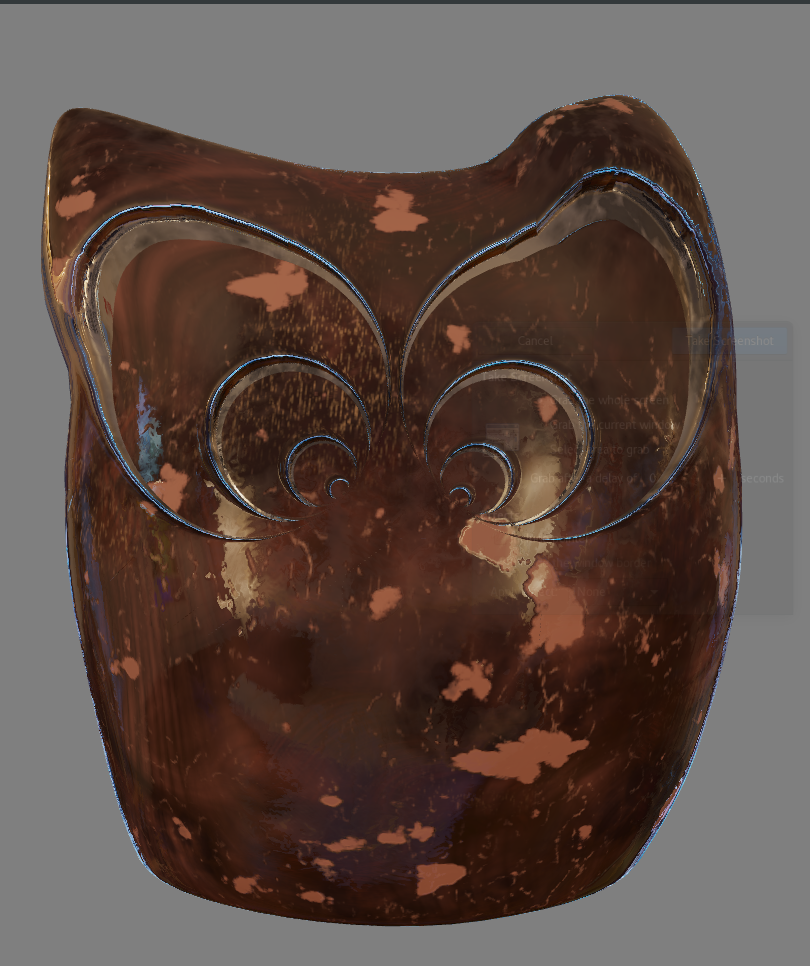
\includegraphics[width=0.49\linewidth]{images/result_shinypose.png}}
 \vfill
  \subfloat[Morphed and metallic]{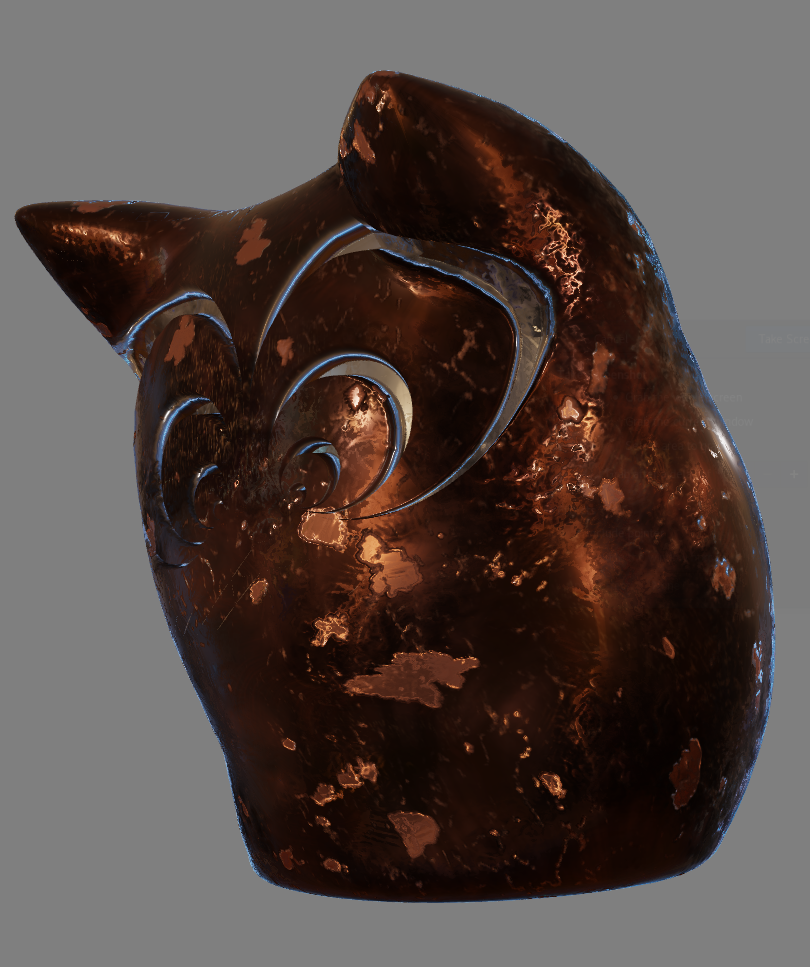
\includegraphics[width=0.49\linewidth]{images/result_metalpose.png}}
 \hfill
 \subfloat[Crazy]{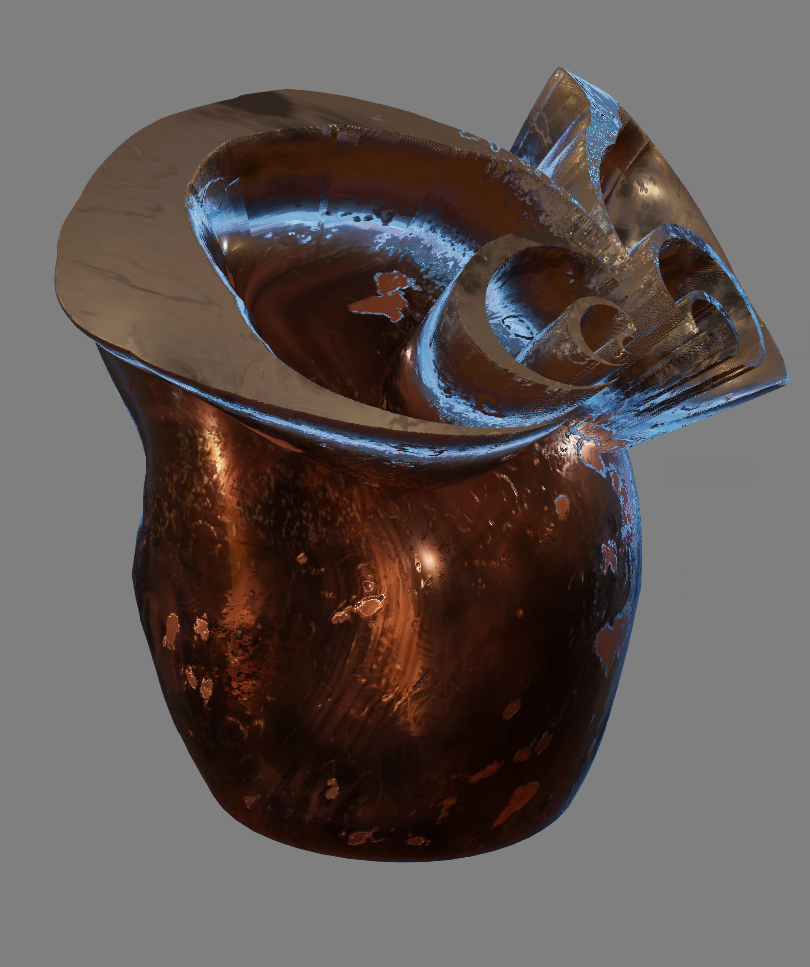
\includegraphics[width=0.49\linewidth]{images/result_crazy.png}}
 \caption{\label{fig:params}Adjusting shader parameters to get different looks.}
\end{figure}

\bibliographystyle{acmsiggraph}
\bibliography{references}


\end{document}
